\chapter{本研究における問題定義と仮説}
\label{issue}

本章では,~\ref{background}章で述べた背景より,本研究における問題とその要件について議論し,
先行研究および提案システムを概説することで本研究で用いるアプローチについて述べる.

\section{本研究における問題定義}
\label{issue:definition}

本研究では、地理的に分散したシステムのステージング環境のための統合環境が未だ整っていないことを問題点とする。

中央システムの形式をとるサービスでは、AWS~\cite{AWS}やGCP~\cite{GCP},Azure~\cite{Azure}といったクラウドサービス等を
活用することで、比較的簡単にステージング環境の構築を行える。
最近では、AWSのEKSやGCPのGKE, AzureのAKSなどクラウドサービス上でフルマネージドなKubernetesクラスタをクリックひとつで
用意することが可能となっている。

対して地理的に分散したシステムでは,ステージング環境の構築は困難である.
P2Pシステムでは個々のノードが地理的に分散し,かつシステムに参加するノード数やノード周辺のネットワーク環境によりシステムの動きが柔軟に変化するため,
ステージング環境はこれらを考慮して構築する必要がある.
地理的かつネットワーク上で論理的に分散したノードを統合的に管理することが困難であるため,そもそも検証作業を行うステージング環境を構築すること自体が困難である.
そこで本研究では,OpenVPNとKubernetesを活用し,地理的かつネットワークにおいて論理的に離れたノードをオーケストレーションすることにより,P2Pシステムの
ステージング環境を提案した.

\section{問題解決における要件}
\label{issue:requirements}
本節では,P2Pシステムのステージング環境に必要な要件を述べる.

\subsection{実際性}
\label{issue:requirements1}
P2Pシステムの検証は,実際のネットワーク上で行う必要がある.
テスト等の論理的検証では不十分である.
P2Pシステムでは,状況に応じてノード同士の関係性・役割が変化し,条件が固定的でないからである.
複雑な条件下での運用が必要であるから,ステージング環境においても,実際に地理的に分散したノードによるネットワークが求められる.

\subsection{統合性}
\label{issue:requirements2}
ステージング環境においては,ある地点から全てのノードを統合的に操作できる必要がある.
現状,アプリケーションの配布・実行・停止等において多大なコミュニケーションコストとヒューマンリソースのオーバーヘッドが問題となっており,
システム内のノードの管理に統合性を持たせることによってこれらのオーバーヘッドを削減する必要がある.

\subsection{拡張性}
\label{issue:requirements3}
ステージング環境では,アプリケーションの修正に伴うアップデートならびにノード数の増加・減少といった変化への柔軟性が必要である.
P2Pシステムは刻一刻と変化するシステムであること.ノードの数によって関係性が変化する.
また,ステージング環境では頻繁なアップデートが予想され,その際に生じるオーバーヘッドの削減が必要である.

\section{先行研究}
\label{issue:previous-research}
P2Pシステムのためのステージング環境の構築手法としては,すでにいくつかの先行研究が存在する.

検証対象のアプリケーションを操作するデバッグエージェントを,あらかじめノード内で起動しておくことにより,アプリケーションの配布や実行,終了を
デバッグクライアントからデバッグエージェントを介して一斉に操作する手法も提案されている.デバッグクライアントからはGUIの操作,ノード間の接続関係の
可視化,ノード間で行われる処理のログ収集などが可能である.

\section{本研究における仮説}
\label{issue:hypothesis}
本研究では~\ref{issue:requirements}章で述べた実際性,統合性,拡張性を担保しながら地理的に分散したシステムのためのステージング環境を構築したい.
そこで,OpenVPNとKubernetesを活用することで,それらの要件を満たしたシステムが構築できるのではないだろうかと考えた.
それぞれの要件に対して,本研究で提案するシステムによる実現が可能であると考えられる点を本節では述べる.

\subsection{実際性}
OpenVPNを活用することで,ネットワーク上で論理的に異なるセグメントに位置するノード同士で疎通が可能なオーバーレイネットワークを構築することができる.
さらに,IP Reachableな条件下であればKubernetesによるクラスタリングが可能である.よって,実際のネットワーク上にステージング環境を構築することが
可能となり,P2Pシステムの検証における実際性が担保されると考えられる.

\subsection{統合性}
Kubernetes自体がオーケストレーションシステムであり,Kubernetesクラスタに参加するワーカーノードはマスターノードからの統合管理が可能である.
そのため本研究では,P2Pシステムに参加するノードをKubernetesクラスタのワーカーノードとして運用することで,マスターノードを経由したアプリケーション
の配布や実行が可能となり,統合性が担保されると考えられる.

\subsection{拡張性}
Kubernetesではアプリケーションをコンテナとして動かすため,ワーカーノード内でコンテナ数を増減したり,コンテナのアップデートを行える.
また,本研究ではKubernetesクラスタ構築時にkubeadmを使用しており,これを用いることで新たなノードをクラスタに参加させることも可能となる.
これによって,修正が重なる可能性のあるステージング環境に必要な拡張性が担保されると考えられる.

\section{提案システム概要}
\label{issue:about-system}
提案システムの概要を述べる.ステージング環境においてP2Pシステムに参加するノード同士を,OpenVPNを利用することで相互に疎通可能な状態にする.
OpenVPNオーバーレイネットワーク上でKubernetesクラスタを構築し,全てのノードをクラスタに参加させる.Kubernetesクラスタ内のマスターノードを
介して,全てのノードに対して操作を行うことができる.

\begin{figure}[htbp]
  \begin{center}
    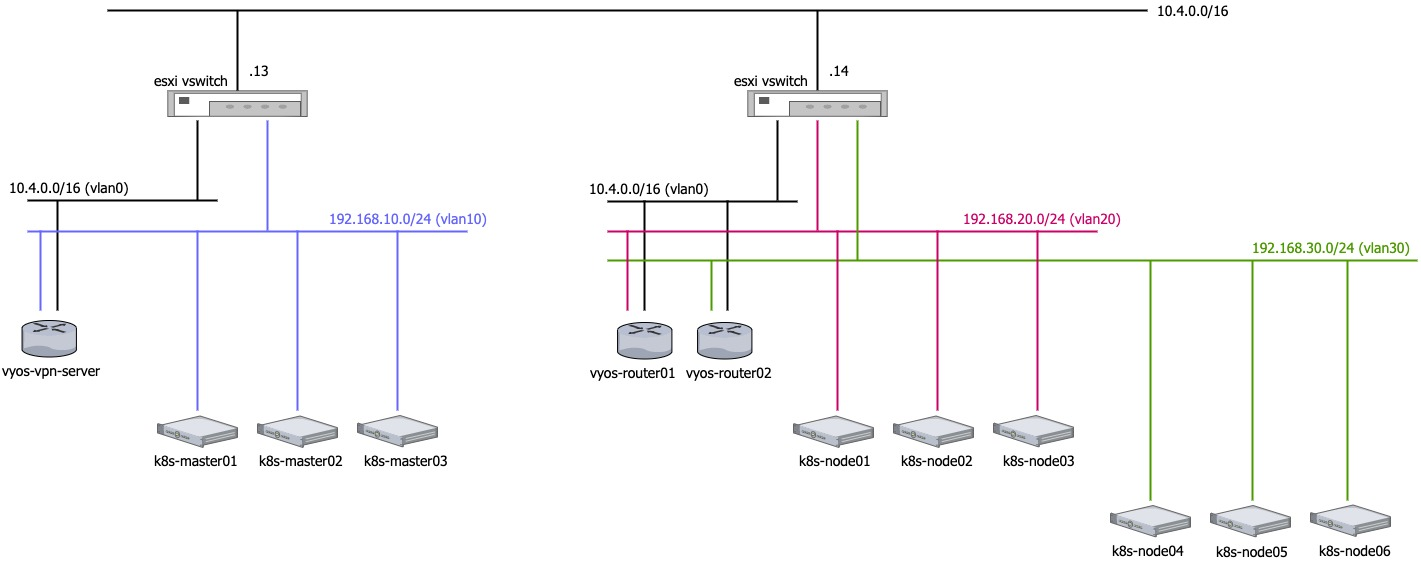
\includegraphics[width=\textwidth]{./figures/system-diagram.jpg}
    \caption{システム概要図}
  \end{center}
\end{figure}

%%% Local Variables:
%%% mode: japanese-latex
%%% TeX-master: "./thesis"
%%% End:
